The distance between the two points is given by
\text{or,} 
\begin{equation}
\begin{aligned}
d = \norm{\vec{P} - \vec{Q}}\\
       = \norm{\begin{pmatrix}
      1\\ 
      -3\\
      4\\
  
    \end{pmatrix} - \begin{pmatrix}
      -4\\ 
      1\\
      2\\
  
    \end{pmatrix}} = \norm{\begin{pmatrix}
      5\\ 
      -4\\
      2\\
  
    \end{pmatrix}}
\\
\implies d = \sqrt{5^2 + (-4)^2 + 2^2}\\
 = 3\sqrt{5}
\end{aligned}
\end{equation}
The  following Python code generates Fig. \ref{fig:line_geo_54_point_distance}
\begin{lstlisting}
solutions/line/geometry/examples/54/codes/point_distance.py
\end{lstlisting}

\begin{figure}[!ht]
\centering
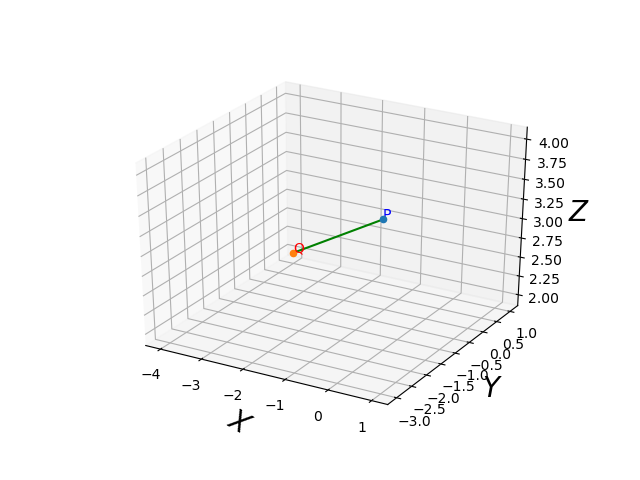
\includegraphics[width=\columnwidth]{./solutions/point_vector/54/figs/point_distance.png}
\caption{Two points and distance between them.}
\label{fig:line_geo_54_point_distance}
\end{figure}
